\documentclass[a4paper,20pt,oneside]{book}
\usepackage[utf8]{inputenc} 
\usepackage[T1]{fontenc} 
\usepackage[nonumberlist]{glossaries} 
\usepackage[english,ngerman]{babel}
\usepackage{float}
\usepackage{graphicx}
\usepackage{longtable}
\usepackage{titlesec}
\usepackage{pdfpages}
\usepackage{glossaries}
\usepackage{listings}
\usepackage{color}
\usepackage{titlepic}
\usepackage{booktabs}
\usepackage{ulem}

\usepackage[DIV=14,BCOR=2mm,headinclude=true,footinclude=false]{typearea}
\definecolor{dkgreen}{rgb}{0,0.6,0}
\definecolor{gray}{rgb}{0.5,0.5,0.5}
\definecolor{mauve}{rgb}{0.58,0,0.82}
\lstset{frame=tb,
	language=bash,
	aboveskip=3mm,
	belowskip=3mm,
	showstringspaces=false,
	columns=flexible,
	basicstyle={\small\ttfamily},
	numbers=none,
	numberstyle=\tiny\color{gray},
	keywordstyle=\color{blue},
	commentstyle=\color{dkgreen},
	stringstyle=\color{mauve},
	breaklines=true,
	breakatwhitespace=true,
	tabsize=3
}

\titleformat{\subparagraph}
{\normalfont\normalsize\bfseries}{\thesubparagraph}{1em}{}
\titlespacing*{\subparagraph}{\parindent}{3.25ex plus 1ex minus .2ex}{.75ex plus .1ex}
\makeglossaries



\begin{document}
	\title{\Huge{\bfseries{Implementierung}}}
	\author{}
	\maketitle
	\clearpage
	
	\tableofcontents
	
	\chapter{Einleitung}
	In diesem Dokument wird die erste Implementierungsphase des Serverless Server Projekts beschrieben.
	
	 Zuerst werden die Probleme und Änderungen im Vergleich zum Entwurf angezeigt.
	
	 Im nächsten Teil werden die Testfälle dargestellt. Sie testen die Klassen, welche die Hauptfunktionalität des Projekts implementieren.
	 \vspace{0.5cm}
	 
	\titlepic{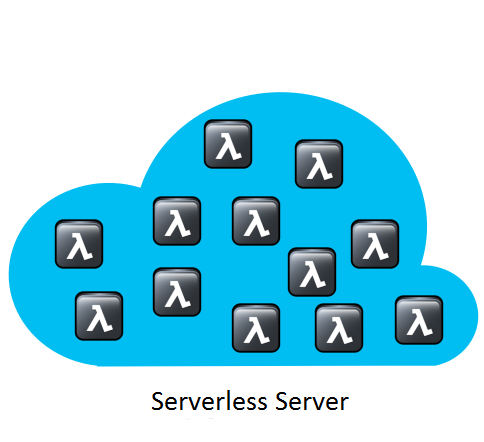
\includegraphics[width=14cm]{Logo.png}}
	\chapter{Probleme und Änderungen am Entwurf}
	In diesem Kapitel werden die Änderungen dokumentiert, die während der ersten Implemetierungsphase gemacht werden. 
	\section{Schichtenmodell}
	Zum verbesserten Verständnis des Systemaufbaus, steht zu Beginn eine Grafik, die das Schichtenmodell beschreibt.
	
	\vspace{0.5cm}
	\includegraphics[width=\textwidth]{schichten.png}
	\section{ApiController} 
	\subsection{RestApiController}
	\vspace{0.5cm}
	\begin{itemize}
	\item Der Name der Klasse ApiController wurde in RestApiController umbenannt.\linebreak
	\item Fast alle Methoden wurden zur besseren Verständlichkeit umbenannt.\linebreak
	\begin{itemize}
	\item  uploadLambda(UploadLambdaRequest): ResponseEntity<UploadLambdaResponse> wurde in postLambda(UploadLambdaRequest): ResponseEntity<UploadLambdaResponse> umbenannt.\linebreak
	\item  executeLambda(nameOfLambda: String, config ExecuteLambdaRequest):\\ ResponseEntity<ExecuteLambdaResponse> wurde in postLambda(nameOfLambda: String, config ExecuteLambdaRequest): ResponseEntity<ExecuteLambdaResponse> umbenannt.\linebreak
	\item  updateLambda(name: String, config: UploadLambdaRequest): ResponseEntity<Void> wurde in putLambda(name: String, config: UploadLambdaRequest): ResponseEntity<Void> umbenannt.\linebreak
	\item showLambda(name: String): ResponseEntity<UploadLambdaRequest> wurde in getLambda(name: String): ResponseEntity<UploadLambdaRequest> umbenannt.\linebreak
	\item generateSubtoken(name: String, expiryDate: String): ResponseEntity<String>
 wurde in  getSubtoken(name: String, expiryDate: String): ResponseEntity<String>
 umbenannt.\linebreak	
	\end{itemize}
	\item Das Attribut tokenCreator: TokenCreator  wurde durch authFacade: AuthFacade umgesetzt. Es folgt aus den Änderungen des Auth Teils. \linebreak
	\item Der Rückgabetyp der Methode putLambda(name: String, config: UploadLambdaRequest): ResponseEntity<Void> wurde zu ResponseEntity<UploadLambdaResponse> verändert.Der Grund ist: token verändert sich nach update, deshalb soll es zurückgegeben sein.\linebreak
	
	\end{itemize}
	\subsection{Exception}
	\subsubsection{ExceptionsHandler} 
	Neue Methoden hinzugefügt, welche Exceptions bearbeiten.
	\section{Auth} 
	
	\subsubsection{AuthFacade}
	
	Hinzugefügt, um die Schnittstelle zur Authentifizierung und Tokengenerierung fest und einheitlich zu machen.	
	
	\vspace{0.5cm}
	\centering
	\begin{tabular}{|l|}
	\hline \\
	AuthFacade \\ \hline 
	\\ \hline \\
	+ generateSubToken(principal:Object, expiryDate:String):String\\ 
   + generateMasterToken(authKey:AuthKey, id:Identifier ):String\\
   + validate(principal:Object):boolean
 \\ \hline
	\end{tabular}
		 
	\vspace{0.5cm}
	\raggedright
	Beschreibung:
	
	Interface zur Definition der Fassade für die Authentifizierung.
	
	\vspace{0.5cm}
	Attribute:
	\begin{itemize}
	\item keine
	\end{itemize}
	
	Methoden:
	\begin{itemize}
	\item generateSubToken(principal:Object, expiryDate:String):String\linebreak
	Deklaration einer Methode zur Generierung von Subtokens (Tokens mit einem expiryDate)
	\item generateMasterToken(authKey:AuthKey, id:Identifier ):String\linebreak
Deklaration einer Methode zur Generierung von MasterTokens (Tokens ohne expiryDate)
	\item validate(principal:Object):boolean\linebreak
	Deklaration einer Methode zur Validierung des AuthKeys.
	\end{itemize}	
	
	\subsubsection{AuthFacadeImpl}
	
	Hinzugefügt als Implementierung der AuthFacade.	
	
	\vspace{0.5cm}
	\centering
	\begin{tabular}{|l|}
	\hline \\
	AuthFacade \\ \hline \\
	-  tokenCreator:TokenCreator\\
	- subtokenCreator:SubtokenCreator \\
	- contentValidator:ContentValidator 
	\\ \hline \\
	+ generateSubToken(principal:Object, expiryDate:String):String\\ 
   + generateMasterToken(authKey:AuthKey, id:Identifier ):String\\
   + validate(principal:Object):boolean
 \\ \hline
	\end{tabular}
		 
	\vspace{0.5cm}
	\raggedright
	Beschreibung:
	
	Implementierung der AuthFacade.
	
	\vspace{0.5cm}
	Attribute:
	\begin{itemize}
	\item tokenCreator:TokenCreator\linebreak
	Verbindung zum TokenCreator zur Generierung von Tokens
	\item subtokenCreator:SubtokenCreator\linebreak
	Verbindung zum SubtokenCreator zur Generierung von Subtokens
	\item contentValidator:ContentValidator \linebreak
	Verbindung zum ContentValidator zur Validierung von Tokens
	\end{itemize}
	
	Methoden:
	\begin{itemize}
	\item generateSubToken(principal:Object, expiryDate:String):String\linebreak
	Generiert einen Subtoken
	\item generateMasterToken(authKey:AuthKey, id:Identifier ):String\linebreak
	Generiert einen Mastertoken
	\item validate(principal:Object):boolean\linebreak
	Validiert einen Token
	\end{itemize}
	
	\subsubsection{ContentValidator}
		
	Hinzugefügt, um Logik aus der AuthFacadeImpl in eine seperate, austauschbare Klasse auszulagern und um eine alleinige Klasse für die Kommunikation	mit der Runtime zu schaffen.
	
	\vspace{0.5cm}
	\centering
	\begin{tabular}{|l|}
	\hline \\
	ContentValidator \\ \hline \\
	-  runtimeController:RuntimeController \\
	\\ \hline \\
   + lambdaExists(name:Identifier):boolean\\
   + validate(accessRights:AccessRights):boolean 
 \\ \hline
	\end{tabular}
		 
	\vspace{0.5cm}
	\raggedright
	Beschreibung:
	
	Klasse zur Validierung von Tokens.
	
	\vspace{0.5cm}
	Attribute:
	\begin{itemize}
	\item runtimeController:RuntimeController\linebreak
	Verbindung zum RuntimeController zum Vergleich von AuthKeys.
	\end{itemize}
	
	Methoden:
	\begin{itemize}
	\item lambdaExists(name:Identifier):boolean\linebreak
	Ruft RuntimeController auf, um die Existenz von einem Lambda mit Identifier zu prüfen.
	\item validate(accessRights:AccessRights):boolean \linebreak
	Ruft RuntimeController auf, um die Existenz von einem Lambda mit Identifier zu prüfen.
	Prüft, ob der AuthKey aus dem Token mit dem AuthKey aus der Runtime übereinstimmt.
	
	\end{itemize}
	
	
	\subsubsection{SubtokenCreator}
	
	Hinzugefügt, um den speziellen Vorgang zum parsen von Daten für den expiryDate auszulagern.	
	
	\vspace{0.5cm}
	\centering
	\begin{tabular}{|l|}
	\hline \\
	SubtokenCreator \\ \hline \\
	-  tokenCreator:TokenCreator \\
	\\ \hline \\
   + generateSubToken(accessRights:AccessRights, expiryDate:String):String
 \\ \hline
	\end{tabular}
		 
	\vspace{0.5cm}
	\raggedright
	Beschreibung:
	
	Klasse zur Erstellung von Subtokens (Tokens mit einem Ablaufdatum)
	
	\vspace{0.5cm}
	Attribute:
	\begin{itemize}
	\item tokenCreator:TokenCreator\linebreak
Verbindung zum TokenCreator zur Erstellung von Tokens.
	\end{itemize}
	
	Methoden:
	\begin{itemize}
	\item generateSubToken(accessRights:AccessRights, expiryDate:String):String\linebreak
	Generiert einen Token mit einem Ablaufdatum.
	\end{itemize}
	
	\subsubsection{JwtAuthTokenFilter}
	keine Änderungen.

	\subsubsection{AccessRights}
	keine Änderungen.
	
	\subsubsection{JwtAuthEntryPoint}
	keine Änderungen.
	
	\subsubsection{JwtAuthProvider}
	keine Änderungen.
	
	\subsubsection{JwtAuthSuccessHandler}
	keine Änderungen.
	
	\subsubsection{JwtAuthTokenStringWrapper}
	keine Änderungen.
	
	\subsubsection{TokenCreator}
	keine Änderungen.

	\subsubsection{AuthenticationConfig}
	keine Änderungen.


		
	\section{Model}
	\subsection{Converter}
	\subsubsection{RequestServerConverter}
	\begin{itemize}
	\item Alle Methoden wurden umbenannt zur besseren Verständlichkeit.\linebreak
	\begin{itemize}
    \item uploadToLambda(uploadRequest: UploadLambdaRequest): Lambda wurde in uploadRequestToLambda(uploadRequest: UploadLambdaRequest): Lambda umbenannt. \linebreak
    \item  executeToConfig(executeRequest: ExecuteLambdaRequest): ExecuteConfig wurde in executeRequestToExecuteConfig(executeRequest: ExecuteLambdaRequest): ExecuteConfig umbenannt. \linebreak
    \item  lambdaToUpload(lambda: Lambda): UploadLambdaRequest wurde in lambdaToUploadRequest(lambda: Lambda): UploadLambdaRequest umbenannt. \linebreak
    
	\end{itemize}
	\item Die Methode  runtimeAttributesRequestToRuntimeAttributes(runtimeAttributesRequest: RuntimeAttributesRequest):RuntimeAttributes wurde hinzugefügt, um von RuntimeAttributesRequest Objekt  ein RuntimeAttributes Objekt zu machen.\linebreak
	\item Die Methode  runtimeAttributesToRuntimeAttributesRequest(runtimeAttributes: RuntimeAttributes): RuntimeAttributesRequest wurde hinzugefügt, um von RuntimeAttributes Objekt  ein RuntimeAttributesRequest Objekt zu machen.\linebreak
	\end{itemize}
	
	\subsection{Exception.Lambda}
	\subsubsection{LambdaDuplicatedNameException}
	keine Änderungen.
	\subsubsection{LambdaNotFoundException}
	keine Änderungen.
	\subsection{Exception.Messages}
	\subsubsection{SemanticRequestException}
	Hinzugefügt um semantische Fehler in JSON Anfrage zu bearbeiten. 
	\subsection{Lambda}
	
	\subsubsection{AuthKey}
	
	Hinzugefügt, um den AuthKey des Lambdas aus der Runtime in ein Objekt zu verpacken.	
	
		\centering
	\begin{tabular}{|l|}
	\hline \\
	AuthKey\\
	\hline \\
    - authKey: String\\
    \hline \\
	\hline 
	\end{tabular}
	
	\raggedright
	\vspace{0.5cm}
	Beschreibung:
	
	Klasse zur Verpackung des AuthKeys der Lambda-Funktion.
	
	\vspace{0.5cm}
	Attribute:
	\begin{itemize}
    \item code: String \linebreak
    Der AuthKey der Funktion als String.
	\end{itemize}
	
	Methoden:
	\begin{itemize}
	\item keine
	\end{itemize}
	\subsubsection{Code}
	keine Änderungen.
	\subsubsection{ExecuteConfig}
	keine Änderungen.
	\subsubsection{Identifier}
	keine Änderungen.	
	\subsubsection{Lambda}
	\begin{itemize}
	\item Das Attribut lambdaImage wurde gelöscht.\linebreak
	\item Das Attribut runtimeAttributes:RuntimeAttributes wurde hinzugefügt.Die Attribute language:Language, libraries:List<Library>, code:Code wurden in runtimeAttributes:RuntimeAttributes übertragen, um bessere Verschachtelung zu realisieren.\linebreak
	 \end{itemize}
	 \subsubsection{RuntimeAttributes}
	
	Hinzugefügt, um Attribute des Lambdas, die in Runtime Tile benutzt wurden, in ein Objekt zu verpacken.	
	
		\centering
	\begin{tabular}{|l|}
	\hline \\
	RuntimeAttributes\\
	\hline \\	
    - language:Language\\
    - libraries:List<Library>\\
    - code:Code\\
    \hline \\
	\hline 
	\end{tabular}
	
	\raggedright
	\vspace{0.5cm}
	Beschreibung:
	
	Klasse zur Verpackung der Attribute der Lambda-Funktion, welche Runtime Teil benutzt.
	
	\vspace{0.5cm}
	Attribute:
	\begin{itemize}
    \item language:Language \linebreak
    Die Sprache der Funktion .
     \item libraries:List<Library> \linebreak
    Die Biblioteken der Funktion .
     \item code:Code \linebreak
    Der Code der Funktion .
	\end{itemize}
	
	Methoden:
	\begin{itemize}
	\item keine
	\end{itemize}
	\subsubsection{Language}
	keine Änderungen.
	\subsubsection{Library}
	keine Änderungen.
	\subsubsection{Parameter}
	keine Änderungen.
	\subsubsection{RunCycles}
	keine Änderungen.
	\subsection{Messages}
	\subsubsection{ExecuteLambdaRequest}
	keine Änderungen.
	\subsubsection{ExecuteLambdaResponse}
	keine Änderungen.
	\subsubsection{RestErrorInfo}
	Das Attribut detail:String wurde gelöscht.
	\subsubsection{RuntimeAttributesRequest}
	
	Hinzugefügt, um JSON Datei verständlicher zu machen.
	
	
		\centering
	\begin{tabular}{|l|}
	\hline \\
	RuntimeAttributesRequest\\
	\hline \\
    - language: String\\
    - libraries: List<String>\\
    - code: String\\
    \hline \\
	\hline 
	\end{tabular}
	
	\raggedright
	\vspace{0.5cm}
	Beschreibung:
	
	Enthält die in Java Attribute geparste RuntimeAttributesRequest Objekt aus JSON Datei, die die Anfrage zum Hochladen enthält.

	
	\vspace{0.5cm}
	Attribute:
	\begin{itemize}
    \item language: String \linebreak
    Die Sprache der Funktion als String.
    \item libraries: List<String>\linebreak
    Die Biblioteken der Funktion .
    \item code: String \linebreak
    Der Code der Funktion als String.
	\end{itemize}
	
	Methoden:
	\begin{itemize}
	\item keine
	\end{itemize}
	\subsubsection{UploadLambdaRequest}
	Die Attribute language:String, libraries:List<String>, code:String wurden in runtimeAttributes:RuntimeAttributesRequest übertragen, weil die Struktur von Lambda Klasse verändert wurde.
	\subsubsection{UploadLambdaResponse}
	keine Änderungen.
	\subsection{ServiceLayer: Service}
	\subsubsection{LambdaManagerFacade}
	\begin{itemize}
	\item Der Name der Schnittstelle LambdaFacade wurde in LambdaManagerFacade zur besseren Verständlichkeit umbenannt.\linebreak
	\item Die Methode authenticate(principal:Object):boolean wurde gelöscht.  Dies folgt aus den Änderungen im Auth Teil.
 \linebreak
 \item Der Rückgabetyp der Methode  deleteLambda(name: String ): String  wurde zu void verändert. Der Grund ist: deleteLambda Methode soll nichts zurückgeben, falls alles gut ist. In dem Fall, wenn was schief läuft, wurde passende Exception geworfen.
 \linebreak
	 \end{itemize}
	\subsubsection{LambdaManagerFacadeImpl}
	\vspace{0.5cm}
	\begin{itemize}
	\item Der Name der Klasse LambdaFacadeImpl wurde in LambdaManagerFacadeImpl zur besseren Verständlichkeit umbenannt. \linebreak
	\item Manche Methoden wurden zur besseren Verständlichkeit umbenannt. Es wurde noch die Lambda und ExecuteConfig Objekterstellung in RestApiController verlegt, um Anfragen allein dort zu behandeln. Deswegen wurden die Anfragen als Parameter in alle Methoden der LambdaManagerFacadeImpl Klasse durch den Lambda und ExecuteConfig Objekten umgesetzt. \linebreak
	\begin{itemize}
	\item   upload(config: UploadLambdaRequest): String  wurde in addLambda(Lambda lambda): String umbenannt.\linebreak
	\item  update(name: String, config: UploadLambdaRequest): String  wurde in updateLambda(String name, Lambda lambda): String umbenannt.\linebreak
	\item   execute(name: String, config: ExecuteLambdaRequest): String  wurde in executeLambda(String name, ExecuteConfig executeConfig): String umbenannt.\linebreak
	
	\end{itemize}
	\item Die Attribute  path: String, maxTimes: int, timeout: long wurden gelöscht. Es wurde wegen der Änderungen in LambdaRuntime Teil gemacht.\linebreak
	\item Das Attribut authHandler: AuthHandler  wurde durch authenticatior: AuthFacade umgesetzt. Es wurde wegen der Änderungen in Auth Teil gemacht. \linebreak
	\item Die Methode authenticate(principal:Object):boolean wurde gelöscht.  
 \linebreak
 \item Der Rückgabetyp der Methode  deleteLambda(name: String ): String  wurde zu void verändert.\linebreak
	\end{itemize}
	
	\subsection{ServiceLayer: Lambdaruntime}
	Allgemeine Änderungen: Die Klassen wurden zur besseren Übersichtlichkeit und Struktur auf die Sub-Pakete images, execution und communication verteilt.
	\subsubsection{RuntimeController}
	\begin{itemize}
		\item Die Erzeugung der Images wurde in eine die Klasse ImageManager verschoben (mit den zugehörigen Methoden). Damit ist RuntimeController nun eine reine Fassade.
		\item Die Rückgabe- und Parametertypen der Methoden buildImage(), rebuildImage() und deleteImage() wurden angepasst.
		\item Neue Methoden:
		\begin{itemize}
			\item lambdaExists(id: Identifier): boolean \\
			Methode leitet die Anfrage and den ImageManager weiter
			\item getAuthKey(id: Identifier): AuthKey \\
			Methode leitet die Anfrage an den ImageManager weiter
			\item getLambda(id: Identifier): Lambda \\
			Methode leitet die Anfrage an den ImageManager weiter
		\end{itemize}
	\end{itemize}
	
	\subsubsection{InstanceManager}
	Die Klasse wurde ins Paket execution verschoben, sonst keine Änderungen.	
	\subsubsection{LambdaInstance}
	Die Klasse wurde ins Paket execution verschoben, sonst keine Änderungen.
	
	\subsubsection{AbstractLambdaFactory}
	Die Klasse wurde ins Paket images verschoben, sonst keine Änderungen.
	\subsubsection{LambdaImage}
	\begin{itemize}
	\item Die Klasse wurde ins Paket images verschoben.
	\item Neues Attribut: authKey: AuthKey
	\end{itemize}
	\subsubsection{Python3LambdaFactory und Python3LambdaImage}
	Die Klassen wurden ins Paket images verschoben, sonst keine Änderungen.
	\subsubsection{OAuthHandler}
	Die Klasse wurde entfernt. Ihre Funktionalität wurde in die Klasse ImageManager integriert.
	\subsubsection{ImageManager}
	\centering
	\vspace{0.5cm}
	\begin{tabular}{|l|}
	\hline \\
	ImageManager \\ \hline \\
	- \underline{instance: ImageManager} \\
	- communicator: RuntimeCommunicator \\
	- factories: List<AbstractLambdaFactory> \\
	- images: List<LambdaImage> \\
	\\ \hline \\
	+ \underline{getInstance(): ImageManager} \\
	+ buildImage(lambda: Lambda): AuthKey \\
	+ rebuildImage(lambda: Lambda): AuthKey \\
	+ deleteImage(id: Identifiert): void \\
	+ init(): void \\
	+ lambdaExists(id: Identifier): boolean \\
	+ getAuthKey(id: Identifier): AuthKey \\
	+ getLambdaImageByIdentifier(id: Identifier): LambdaImage \\
	- loadImageFactories(): void
 	\\ \hline
	\end{tabular}
		 
	\vspace{0.5cm}
	\raggedright
	Beschreibung:
	
	Eine neue Klasse zur Verwaltung von Images, die Erzeugung von Images in RuntimeController und die Authentifizierung in OAuthHandler wurden in diese Klasse verschoben.
	
	\vspace{0.5cm}
	Attribute:
	\begin{itemize}
	\item instance: ImageManager
	\linebreak Instanz für das Singleton-Pattern
	\item communicator: RuntimeCommunicator
	\linebreak Referenz auf den Kommunikator
	\item factories: List<AbstractLambdaFactory>
	\linebreak Die Fabriken zur Produktion der Images
	\item images: List<LambdaImage>
	\linebreak Liste der vorhandenen Images
	\end{itemize}
	
	Methoden:
	\begin{itemize}
	\item getInstance(): ImageManager
	\linebreak gibt die einzige Instanz von ImageManager zurück
	\item buildImage(lambda: Lambda): AuthKey
	\linebreak erzeugt ein Image
	\item rebuildImage(lambda: Lambda): AuthKey
	\linebreak baut ein Image neu
	\item deleteImage(id: Identifier): void
	\linebreak löscht ein Image
	\item init(): void
	\linebreak initialisiert den ImageManager
	\item lambdaExists(id: Identifier): boolean
	\linebreak gibt zurück, ob das Image vorhanden ist
	\item getAuthKey(id: Identifier): AuthKey
	\linebreak gibt den zu Identifier gehörigen AuthKey zurück
	\item getLambdaImageByIdentifier(id: Identifier): LambdaImage
	\linebreak gibt das zum Identifier gehörige LambdaImage zurück
	\item loadImageFactories(): void
	\linebreak lädt die Fabriken zur Erzeugung der LambdaImages
	\end{itemize} 
	
	\subsubsection{LambdaNotFoundException}
	\centering
	\begin{tabular}{|l|}
	\hline \\
	LambdaNotFoundException \\ \hline \\
	\\ \hline \\
 	\\ \hline
	\end{tabular}
	
	\subsubsection{TimeExceededException}
	\centering
	\begin{tabular}{|l|}
	\hline \\
	TimeExceededException \\ \hline \\
	\\ \hline \\
 	\\ \hline
	\end{tabular}
		 
	\vspace{0.5cm}
	\raggedright
	Beschreibung:
	Exception-Klasse für den Fall, das auf nicht vorhandene Lambdas zugegriffen wird.
	
	
	\subsubsection{CommandType}
	Die Klasse wurde ins Paket communication verschoben, sonst keine Änderungen.
	\subsubsection{RuntimeCommand}
	Die Klasse wurde ins Paket communication verschoben, sonst keine Änderungen.
	\subsubsection{RuntimeConnectException}
	Die Klasse wurde ins Paket communication verschoben, sonst keine Änderungen.
	\subsubsection{RuntimeCommunicator}
	Die Klasse wurde ins Paket communication verschoben, sonst keine Änderungen.
	 
	\section{Application}
	keine Änderungen.
	
	
\chapter{Testfälle}

\section{Auth}

Die Authentifizierung besteht aus zwei Teilen. Das Kapitel "\ Spring Security Tests"\  beschreibt durch Tests das Zusammenspiel mit Spring Security, welches vor dem Eintritt in die LambdaManagerFassade passiert. Hier wird das übergebene JSON Webtoken auf Syntax und zeitliche Gültigkeit geprüft. 

		Der zweite Teil hinter der Fassade 'Validation Tests"\ geschieht mit Zusammenspiel der Runtime und der Fassadenklasse. Diese prüfen die Werte aus dem Token (z.B. AuthKey) mit den zugehörigen Images und erlauben Zutritt bei korrekten Werten. 
		
		"Token Generation Tests"\  widmet sich allein der Generierung von Tokens.

\subsection{Spring Security Tests}
Die "\ Spring Security Tests"\ werden mithilfe von JUnit in einem separaten Projekt durchgeführt, nachdem der Server hochgefahren ist. Grund dafür ist die komplexe Spring Testing Umgebung, die lange, intensive Einarbeitung benötigt, welche nicht gegeben ist. 

\subsection{Validation Tests}
Die "Validation Tests"\ werden mithilfe von JUnit durchgeführt. 

\subsubsection{Test: validateMasterToken}
"validateMasterToken"\ testet Validierung einen gültigen Master-Token.

\begin{itemize}
\item Vorbedingung\linebreak
Ein gültiger Master-JWT wird als ein Objekt AccessRights von dem aufrufenden Modul übergeben. Die Lambda mit dem entsprechenden AccessKey existiert.
\item Beschreibung\linebreak
Die Methode validate wird mit dem JWT als Parameter aufgerufen, und es wird geprüft, ob sie "true" zurückgibt.
\item Nachbedingung\linebreak
Der  Master-JWT wird validiert und "true" wird zurückgegeben. Der JWT bleibt unverändert.
\end{itemize}
\subsubsection{Test: validateSubtoken}
"validateSubtoken"\ testet Validierung einen gültigen Subtoken.

\begin{itemize}
\item Vorbedingung\linebreak
Ein nicht abgelaufener Sub-JWT wird als ein Objekt AccessRights von dem aufrufenden Modul übergeben. Die Lambda mit dem entsprechenden AccessKey existiert.
\item Beschreibung\linebreak
Die Methode validate wird mit dem JWT als Parameter aufgerufen, und es wird geprüft, ob sie "true" zurückgibt.
\item Nachbedingung\linebreak
Der  Sub-JWT wird validiert und "true" wird zurückgegeben. Der JWT bleibt unverändert.
\end{itemize}
\subsubsection{Test: validateInvalidSubtoken}
"validateInvalidSubtoken"\ testet Validierung einen ungültigen Subtoken.

\begin{itemize}
\item Vorbedingung\linebreak
Ein nicht abgelaufener Sub-JWT wird als ein Objekt AccessRights von dem aufrufenden Modul übergeben. Die Lambda mit dem entsprechenden AccessKey existiert nicht.
\item Beschreibung\linebreak
Die Methode validate wird mit dem JWT als Parameter aufgerufen, und es wird geprüft, ob sie eine Exception zurückgibt.
\item Nachbedingung\linebreak
Eine Exception wird zurückgegeben.
\end{itemize}
\subsubsection{Test: validateSubtokenPastDate}
"validateSubtokenPastDate"\ testet Validierung einen abgelaufenen Subtoken.
\begin{itemize}
\item Vorbedingung\linebreak
Ein abgelaufener Sub-JWT wird als ein Objekt AccessRights von dem aufrufenden Modul übergeben. Die Lambda mit dem entsprechenden AccessKey existiert.
\item Beschreibung\linebreak
Die Methode validate wird mit dem JWT als Parameter aufgerufen, und es wird geprüft, ob sie "false" zurückgibt.
\item Nachbedingung\linebreak
"False" wird zurückgegeben.
\end{itemize}
\subsection{Token Generation Tests}
Die "Validation Tests"\ werden mithilfe von JUnit durchgeführt. 
\subsubsection{Test: getMasterToken}
"getMasterToken"\ testet die korrekte Erstellung von MasterToken mit korrekten Eingaben.

\begin{itemize}
\item Vorbedingung\linebreak
Gültige Parameter AuthKey und Identifier werden von dem aufrufenden Modul gegeben. Ein gültiger AuthKey ist ein Objekt AuthKey mit Inhalt Runtime ID als String von der erstellten Lambda-Funktion. Ein gültiger Identifier ist ein Objekt Identifier mit Inhalt Name der zu erstellenden Lambda-Funktion als String. 
\item Beschreibung\linebreak
Der resultierende JWT als String wird nach dem Aufruf der AuthFassadeImpl mit Methode generateMasterToken(auth, id) (mit vorher erstellten Objekten) mit einem extern erstellten JWT mit denselben Parametern verglichen.
\item Nachbedingung\linebreak
Ein gültiger JWT (ohne Auslaufdatum) wurde erstellt und zurückgegeben. Die Parameter vom Anfang bleiben unverändert.
\end{itemize}
	

\subsubsection{Test: getSubToken}
"getSubToken"\ testet die korrekte Erstellung von JWT mit korrekten Eingaben.
\begin{itemize}
\item Vorbedingung\linebreak
Ein gültiges AccessRights und ein gültiges, in der Zukunft liegendes Datum im Format yyyy-mm-dd hh-mm-ss werden übergeben.
\item Beschreibung\linebreak
Ein AccessRights Objekt mit gültigen Parametern wird erstellt. Dann wird generateSubToken(accessRights, expiryDate) (expiryDate ist ein gültiger String) aufgerufen. Der zurückgegebene wird dann mit einem extern erstellten JWT verglichen.
\item Nachbedingung\linebreak
Ein gültiger JWT mit Auslaufdatum wurde erstellt und zurückgegeben. Die Parameter vom Anfang bleiben unverändert.
\end{itemize}


\newpage
\section{RestApiController}
Hier werden Tests dargestellt, die Spezifikation der RestApiController-Klasse prüfen. Alle Tests werden mithilfe von JUnit durchgeführt.

\subsection{Test: postValidLambda}
Hier ist Hochladen von Lambda mit korrekter Anfrage eines Nutzers geprüft. 
\begin{itemize}
	\item Vorbedingung \linebreak
	Lambda, die ein Nutzer hochladen will, muss nicht im System sein, Anfrage muss korrekt sein.
	\item Beschreibung \linebreak
	Zuerst wird Existenz von Lambda im System geprüft. Dannach wird entsprechenden postLambda-Befehl von RestApiController aufgeruft. Endlich werden Nachbedingungen mithilfe von  entsprechenden Methoden von RestApiController geprüft.
	\item Nachbedingung \linebreak
	Lambda muss schon im System sein und kann aktualisiert, gezeigt, gelöscht, ausgeführt werden und Subtoken kann erstellt werden, damit andere Nutzer, die diesen Subtoken besitzen, entsprechende Lambda benutzen können.
\end{itemize}

Hier wird gezeigt, was bei der Aufruf der postLambda-Methode zurückgegeben wird.

\vspace{0.5cm}
	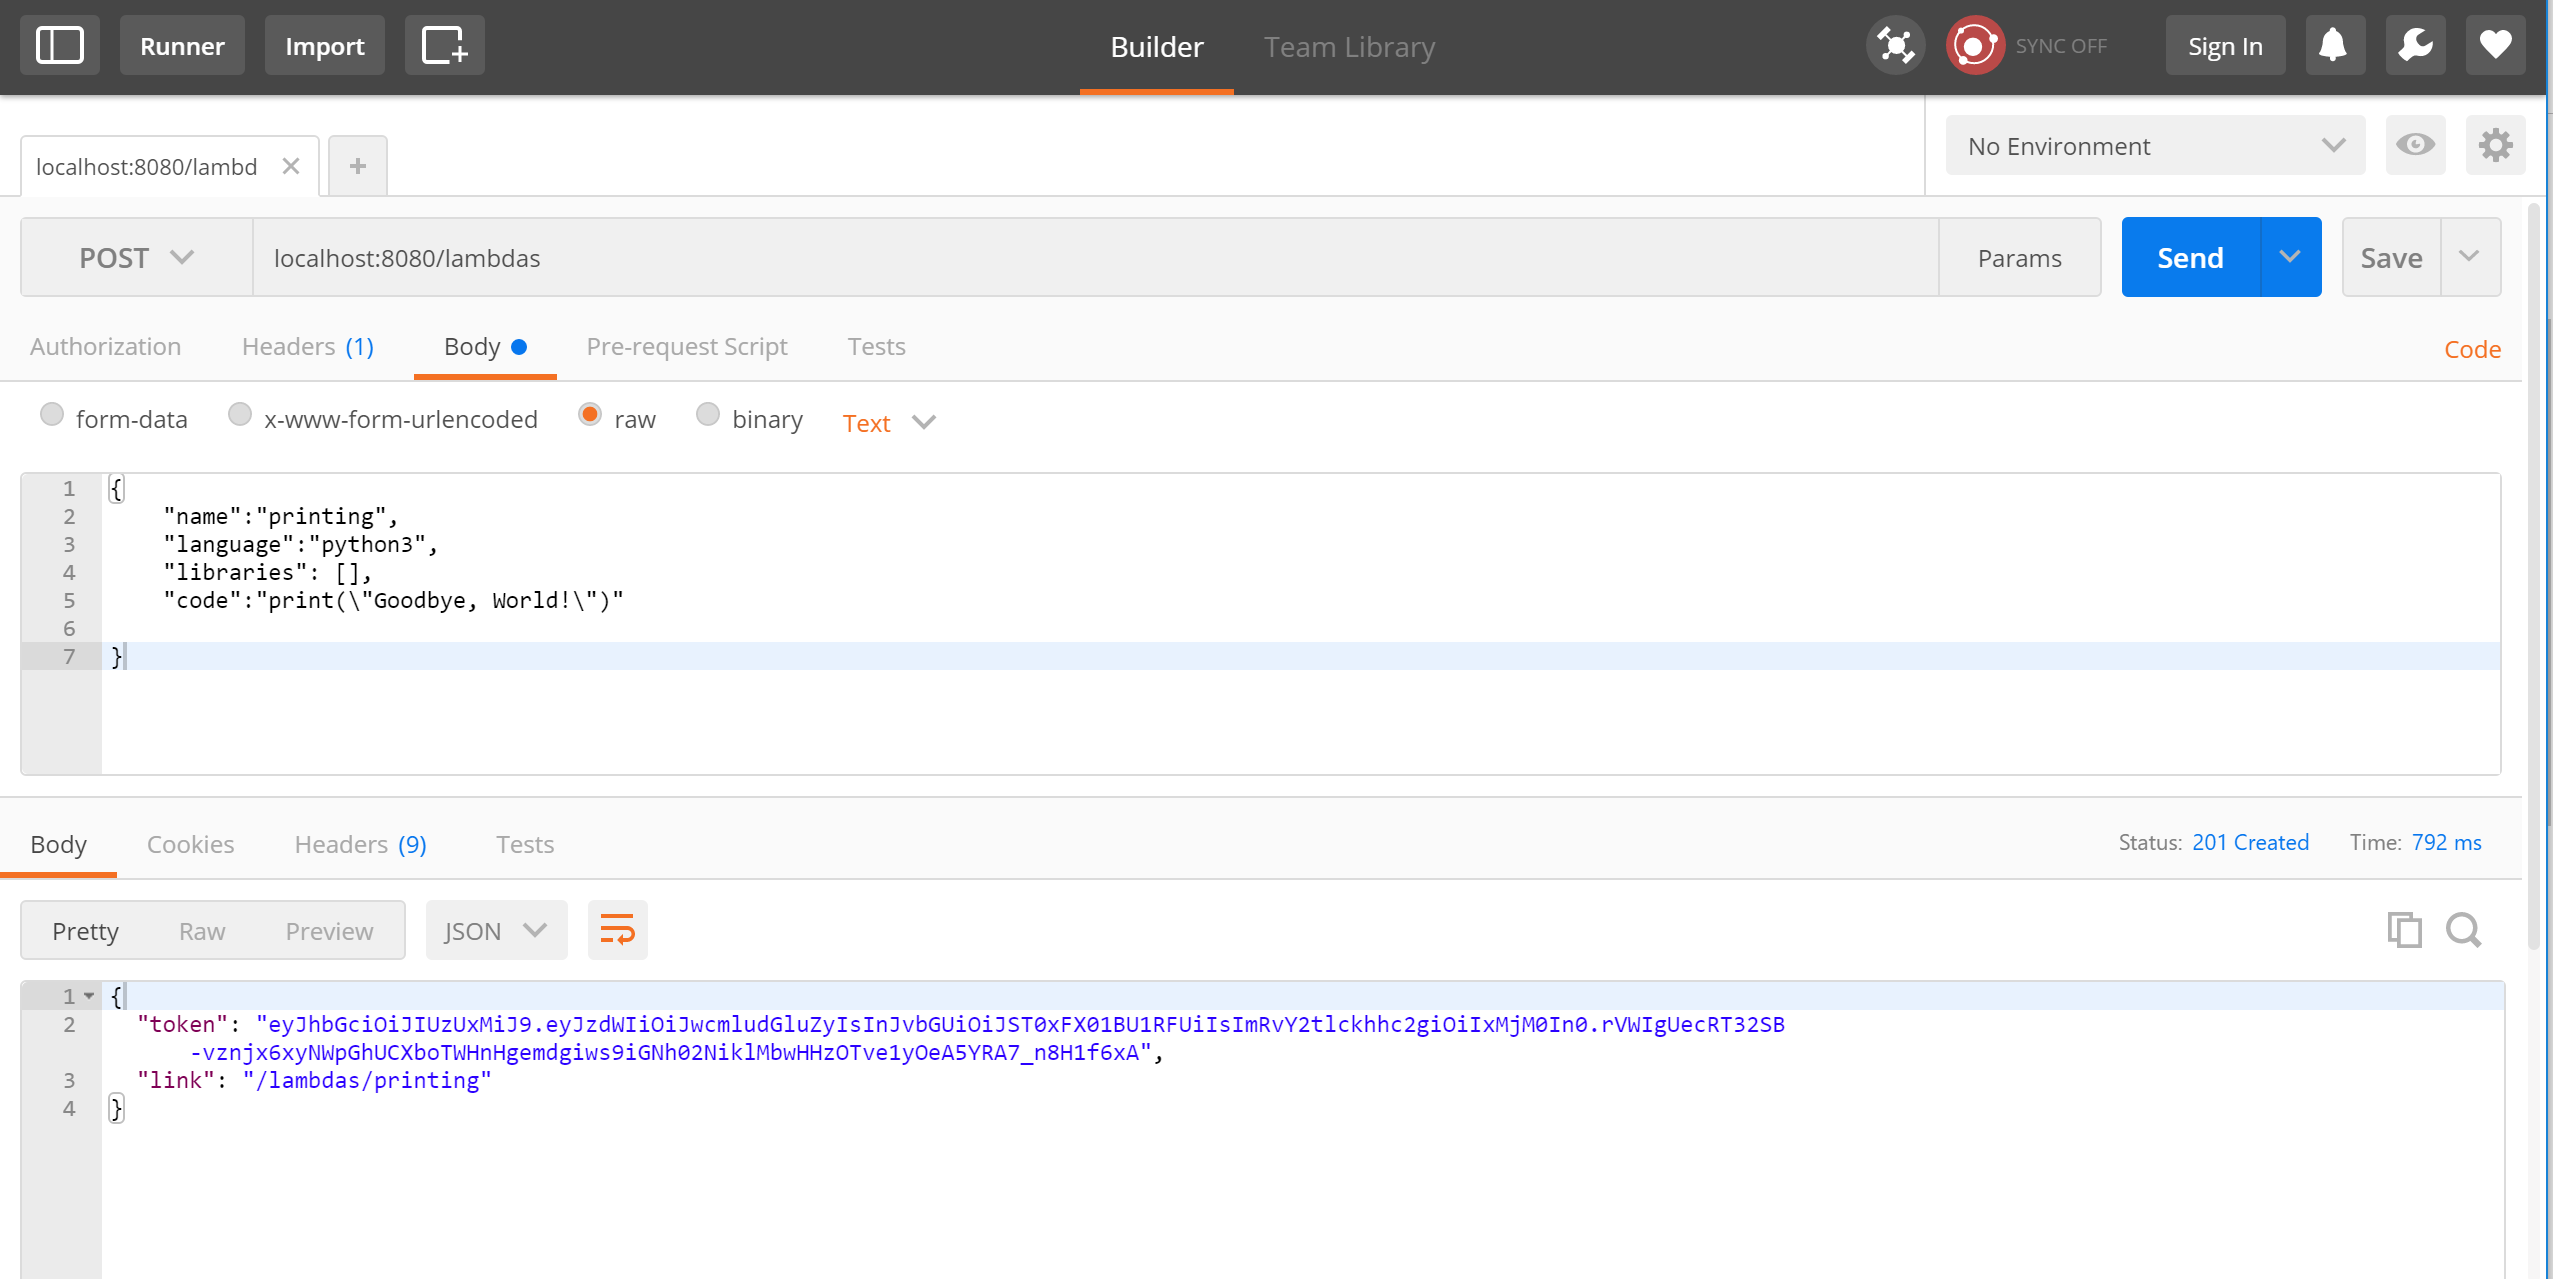
\includegraphics[width=\textwidth]{postmanEx.png}
	
\subsection{Test: postExistedLambda}
Hier ist Hochladen von Lambda geprüft, die schon im System existiert.
\begin{itemize}
	\item Vorbedingung \linebreak
	Lambda muss schon im System sein.
	\item Beschreibung
	Zuerst wird Existenz von Lambda im System geprüft. Dannach wird entsprechenden postLambda-Befehl von RestApiController aufgeruft. Endlich werden Nachbedingungen mithilfe von  entsprechenden Methoden von RestApiController geprüft.
	\item Nachbedingung
	Lambda, die Nutzer hochladen will, muss nicht im System sein. RestApiController muss Antwort mit Status "BAD REQUEST"\ schicken.
\end{itemize}
\subsection{Test: postInvalidLambda}
Hier ist Hochladen von Lambda geprüft, wenn Nutzer unkorrekte Anfrage schickt (z.B. unkorrekte Name von Lambda).
\begin{itemize}
	\item Vorbedingung \linebreak
	Lambda, die ein Nutzer hochladen will, muss nicht im System sein, Anfrage muss korrekt sein.
	\item Beschreibung \linebreak
	Zuerst wird Existenz von Lambda im System geprüft. Dannach wird entsprechenden postLambda-Befehl von RestApiController aufgeruft. Endlich werden Nachbedingungen mithilfe von  entsprechenden Methoden von RestApiController geprüft.
	\item Nachbedingung \linebreak
	Lambda muss nicht im System sein, d.h. Lambda kann nicht aktualisiert, gezeigt, gelöscht, ausgeführt werden und Subtoken kann nicht erstellt werden, damit andere Nutzer, die diesen Subtoken besitzen, entsprechende Lambda benutzen können.
\end{itemize}
 \subsection{Test: postLambdaValidExecute}
 Hier ist Ausführung von Lambda geprüft, wenn Nutzer korrekte Anfrage schickt.
 \begin{itemize}
 	\item Vorbedingung \linebreak
 	Lambda, die ein Nutzer ausführen will, muss im System sein, Anfrage muss korrekt sein.
 	\item Beschreibung \linebreak
 	Zuerst wird Existenz von Lambda im System geprüft. Dannach wird entsprechenden postLambda-Befehl von RestApiController aufgeruft. Endlich werden Nachbedingungen mithilfe von  entsprechenden Methoden von RestApiController geprüft.
 	\item Nachbedingung \linebreak
 	Lambda muss im System bleiben, d.h. Lambda kann aktualisiert, gezeigt, gelöscht, noch mal ausgeführt werden und Subtoken kann erstellt werden, damit andere Nutzer, die diesen Subtoken besitzen, entsprechende Lambda benutzen können.
 \end{itemize}  
 \subsection{Test: postLambdaInValidExecute}
Hier ist Ausführung von Lambda geprüft, wenn Nutzer unkorrekte Anfrage schickt (z.B. Eingabe, dessen Typ keine Signatur von Lambda passt).
\begin{itemize}
	\item Vorbedingung \linebreak
	Lambda, die ein Nutzer ausführen will, muss im System sein, Anfrage muss unkorrekt sein.
	\item Beschreibung \linebreak
	Zuerst wird Existenz von Lambda im System geprüft. Dannach wird entsprechenden postLambda-Befehl von RestApiController aufgeruft. Endlich werden Nachbedingungen mithilfe von  entsprechenden Methoden von RestApiController geprüft.
	\item Nachbedingung \linebreak
	Lambda muss im System bleiben, d.h. Lambda kann aktualisiert, gezeigt, gelöscht, noch mal ausgeführt werden und Subtoken kann erstellt werden, damit andere Nutzer, die diesen Subtoken besitzen, entsprechende Lambda benutzen können.
\end{itemize}  
 
\newpage
\section{LambdaManagerFacadeImpl}
Hier werden Tests dargestellt, die Spezifikation der LambdaManagerFacadeImpl-Klasse prüfen. Alle Tests werden mithilfe von JUnit durchgeführt.

\subsection{Test: addValidLambda}
Hier ist Ergänzung von Lambda ins System geprüft, wenn Lambda-Obkekt korrekte Attribute besitzt (z.B. korrekter Name, Sprache).
\begin{itemize}
	\item Vorbedingung \linebreak
	Lambda muss nicht im System sein, Lambda-Objekt muss korrekte Attributen besitzen.
	\item Beschreibung \linebreak
	Zuerst wird Existenz von Lambda im System geprüft. Dannach wird addLambda-Befehl von LambdaManagerFacadeImpl aufgeruft. Endlich werden Nachbedingungen mithilfe von  entsprechenden Methoden von LambdaManagerFacadeImpl geprüft.
	\item Nachbedingung \linebreak
	Lambda muss im System sein, d.h. Lambda kann aktualisiert, gezeigt, gelöscht, ausgeführt werden.
\end{itemize}
\subsection{Test: addExistedLambda}
Hier ist Ergänzung von Lambda ins System geprüft, wenn Lambda schon im System existiert.
\begin{itemize}
	\item Vorbedingung \linebreak
	Lambda muss im System sein.
	\item Beschreibung \linebreak
	Zuerst wird Existenz von Lambda im System geprüft. Dannach wird addLambda-Befehl von LambdaManagerFacadeImpl aufgeruft. Endlich wartet man auf entspreche Ausnahme.
	\item Nachbedingung \linebreak
	Es muss eine Ausnahme geworfen werden.
\end{itemize}
\subsection{Test: executeValidLambda}
Hier ist Aufführung von Lambda ins System geprüft, wenn Lambda im System existiert.
\begin{itemize}
	\item Vorbedingung \linebreak
	Lambda muss im System sein.
	\item Beschreibung \linebreak
	Zuerst wird Existenz von Lambda im System geprüft. Dannach wird executeLambda-Befehl von LambdaManagerFacadeImpl aufgeruft. Endlich werden Nachbedingungen mithilfe von  entsprechenden Methoden von LambdaManagerFacadeImpl geprüft.
	\item Nachbedingung \linebreak
	Lambda muss im System bleiben, d.h. Lambda kann aktualisiert, gezeigt, gelöscht, noch mal ausgeführt werden.
\end{itemize}
\subsection{Test: executeInvalidLambda}
Hier ist Aufführung von Lambda ins System geprüft, wenn Lambda im System nicht  existiert.
\begin{itemize}
	\item Vorbedingung \linebreak
	Lambda muss nicht im System sein.
	\item Beschreibung \linebreak
	Zuerst wird Existenz von Lambda im System geprüft. Dannach wird executeLambda-Befehl von LambdaManagerFacadeImpl aufgeruft. Endlich wartet man auf entspreche Ausnahme.
	\item Nachbedingung \linebreak
	Es muss eine Ausnahme geworfen werden.
\end{itemize}

\newpage
  \section{LambdaRuntime} 
\subsection{Test: testUpload}			
	"testUpload" testet das Hochladen von einer Test-Lambda und das Bauen von ihrem Image.

\begin{itemize}
\item Vorbedingung\linebreak
Die Lambda existiert noch nicht im System.
\item Beschreibung\linebreak
Erstmal wird geprüft, ob die Lambda im System existiert, und falls sie existiert, gibt der Test "false" zurück. Dann wird ein Image für diese Lambda gebaut, und wird geprüft, ob die Lambda jetzt existiert. Anschließend wird geprüft, ob die Lambda aufrufbar ist, indem sie aufgerufen wird.
\item Nachbedingung\linebreak
Die Lambda existiert im System und ist aufrufbar.
\end{itemize}

\subsection{Test: testUpdate}			
	"testUpdate" testet das Aktualisieren von einer existierenden Test-Lambda und das Umbauen von ihrem Image.

\begin{itemize}
\item Vorbedingung\linebreak
Die Lambda existiert bereits im System.
\item Beschreibung\linebreak
Erstmal wird ein Image für die Test-Lambda gebaut. Dann wird das Image für diese Lambda umgebaut (rebuildImage), und wird geprüft, ob die Lambda jetzt immer noch existiert. Anschließend wird geprüft, ob die Lambda aufrufbar ist, indem sie aufgerufen wird.
\item Nachbedingung\linebreak
Die Lambda existiert immer noch im System und ist aufrufbar.
\end{itemize}

\subsection{Test: testDelete}			
	"testDelete" testet das Löschen von einer existierenden Test-Lambda.

\begin{itemize}
\item Vorbedingung\linebreak
Die Lambda existiert bereits im System.
\item Beschreibung\linebreak
Erstmal wird ein Image für die Test-Lambda gebaut. Dann wird das Image für diese Lambda gelöscht, und wird geprüft, ob die Lambda jetzt nicht mehr existiert. Anschließend wird geprüft, ob die Lambda aufrufbar ist, indem sie aufgerufen wird (eine Exception ist an der Stelle erwartet).
\item Nachbedingung\linebreak
Die Lambda existiert nicht mehr im System und ist nicht mehr aufrufbar.
\end{itemize}

\subsection{Test: testRun}			
	"testRun" testet das Ausführen von einer existierenden Test-Lambda.

\begin{itemize}
\item Vorbedingung\linebreak
Die Lambda existiert bereits im System.
\item Beschreibung\linebreak
Erstmal wird ein Image für die Test-Lambda gebaut. Dann wird getestet, ob das Image für diese Lambda aufgerufen werden kann. Anschließend wird geprüft, ob die Lambda immer noch existiert und aufrufbar ist, indem sie noch mal aufgerufen wird.
\item Nachbedingung\linebreak
Die Lambda existiert immer noch im System und kann noch mal aufgerufen werden.
\end{itemize}
\subsection{Test: testRunNotExisting}			
	"testRunNotExisting" testet das Ausführen von einer nicht-existierenden Test-Lambda.

\begin{itemize}
\item Vorbedingung\linebreak
Die Lambda existiert nicht im System.
\item Beschreibung\linebreak
Ein Image wird für die Lambda NICHT gebaut (sie existiert also nicht im System), und es wird getestet, ob das Image für diese Lambda aufgerufen werden kann (eine Exception ist erwartet). Anschließend wird geprüft, ob die Lambda immer noch nicht existiert.
\item Nachbedingung\linebreak
Die Lambda existiert immer noch nicht im System.
\end{itemize}

\subsection{Test: testStatelessness}			
	"testStatelessness" prüft, ob eine Test-Lambda, die mehrmals ausgeführt wird, immer das gleiche Ergebnis zurückliefert.

\begin{itemize}
\item Vorbedingung\linebreak
Die Lambda existiert im System.
\item Beschreibung\linebreak
Eine Test-Lambda wird angelegt, die versucht es, eine Datei anzulegen, und wenn die Datei noch nicht existiert, gibt die Lambda "created" zurück, sonst "already exists". In dem Testfall wird es in einer for-Schleife 20-Mal geprüft, ob die Test-Lambda jedes Mal "created" zurückgibt.
\item Nachbedingung\linebreak
Die Lambda gibt in jeder Ausführung das gleiche Ergebnis zurück.
\end{itemize}
	\chapter{Bedienungsanleitung des Programms}
	\section{Programm starten}
	Das Programm muss bereits auf einem Server laufen, um Befehle empfangen und ausführen zu können. Die REST-konforme Befehle werden direkt auf diesen Server in curl-Format geschickt, mit einer JSON-Datei als body. Als Antwort wird ebenfalls eine JSON-Datei erhalten. 
	\section{Lambda hochladen}	
	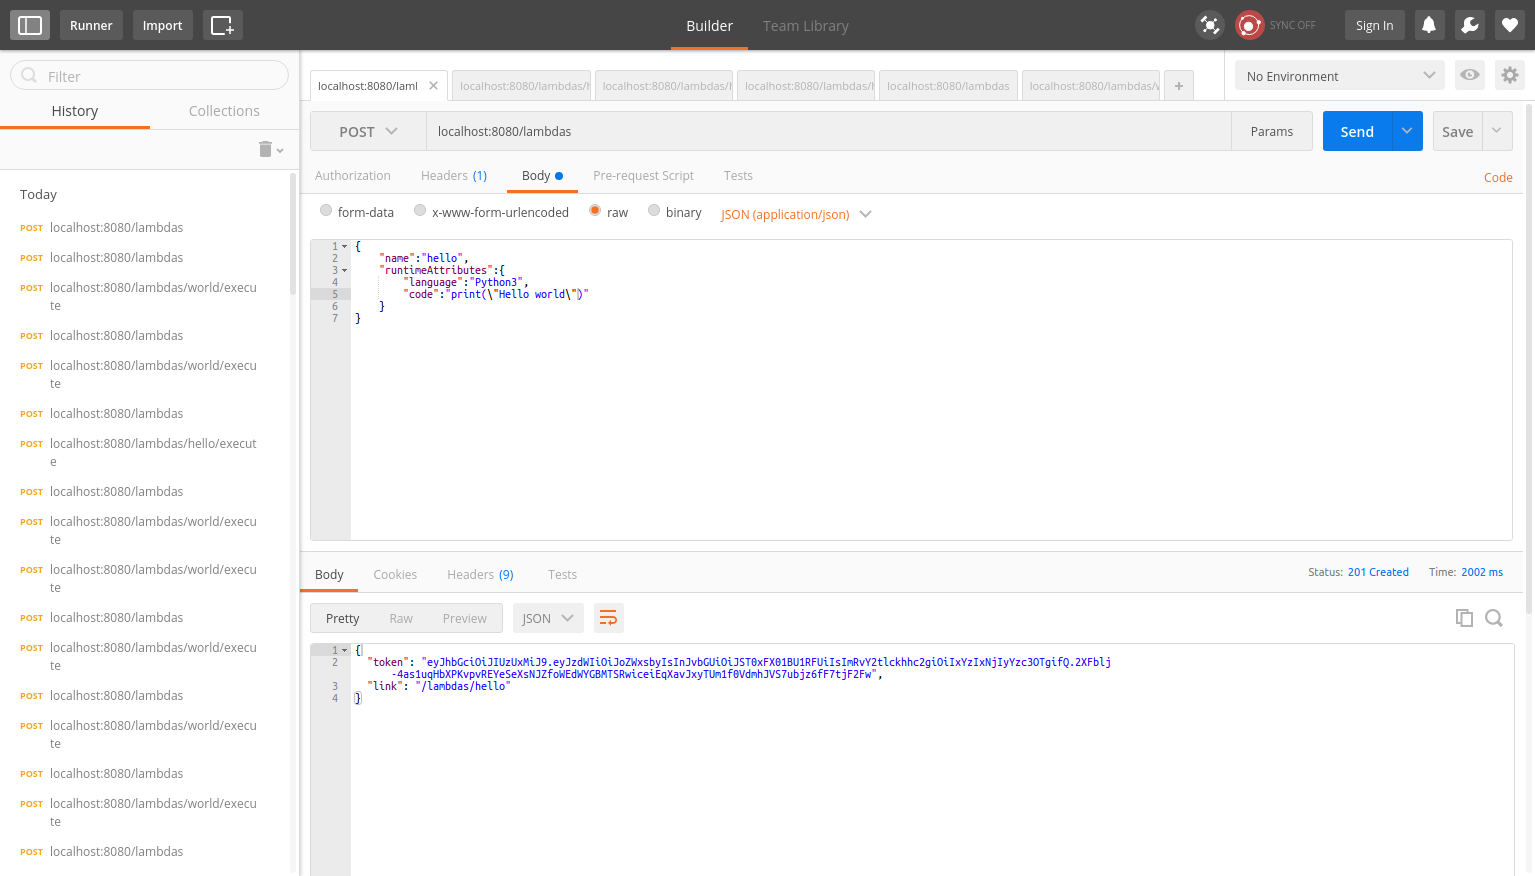
\includegraphics[width=\textwidth]{upload.png}
	\section{Lambda aktualisieren}
	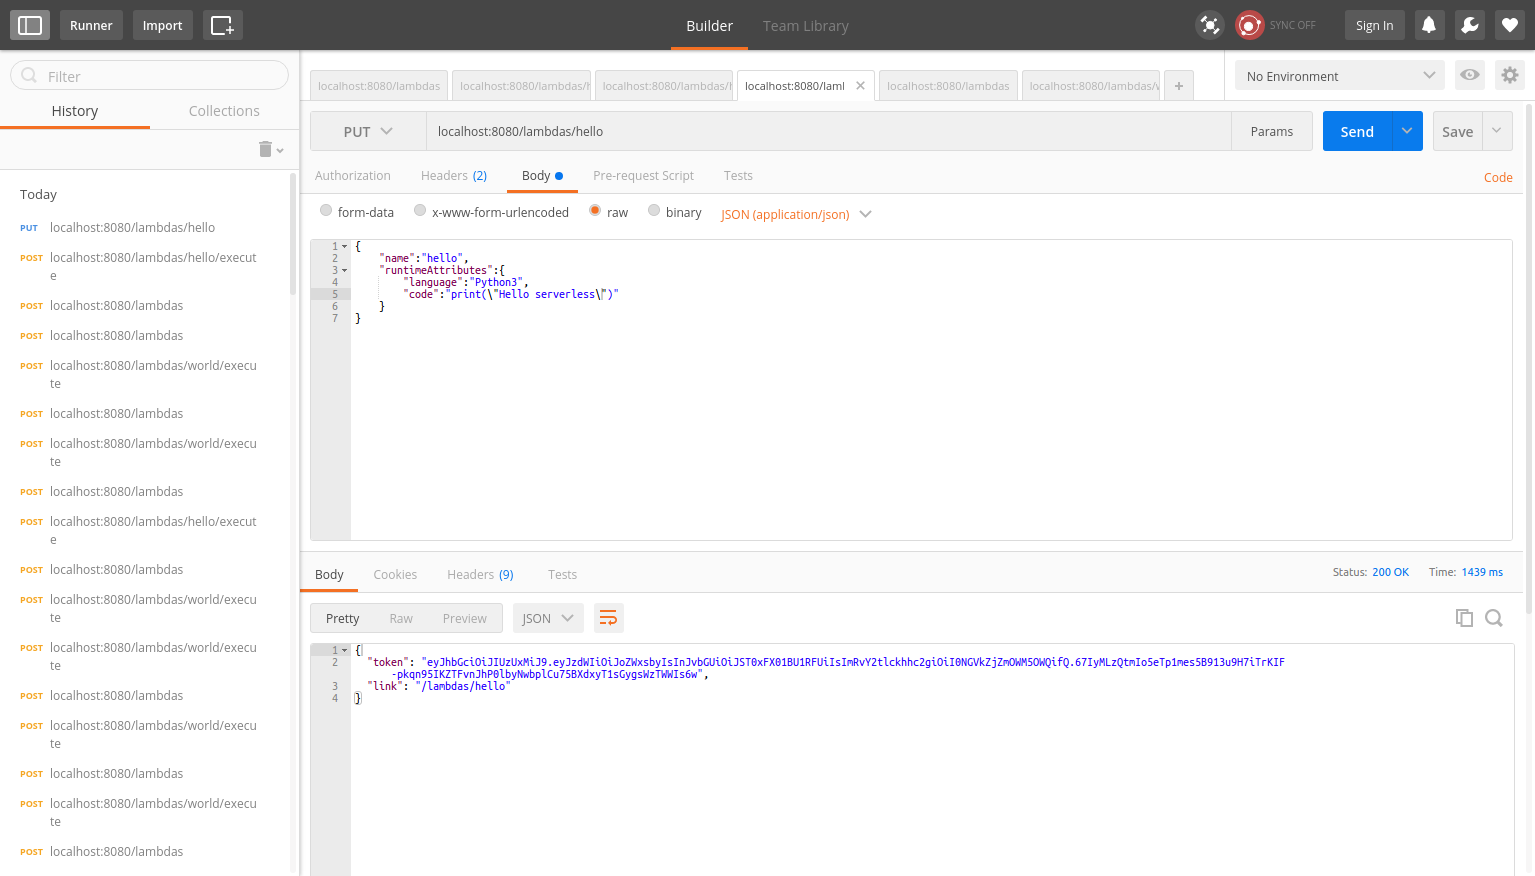
\includegraphics[width=\textwidth]{update.png}
	\section{Lambda löschen}
	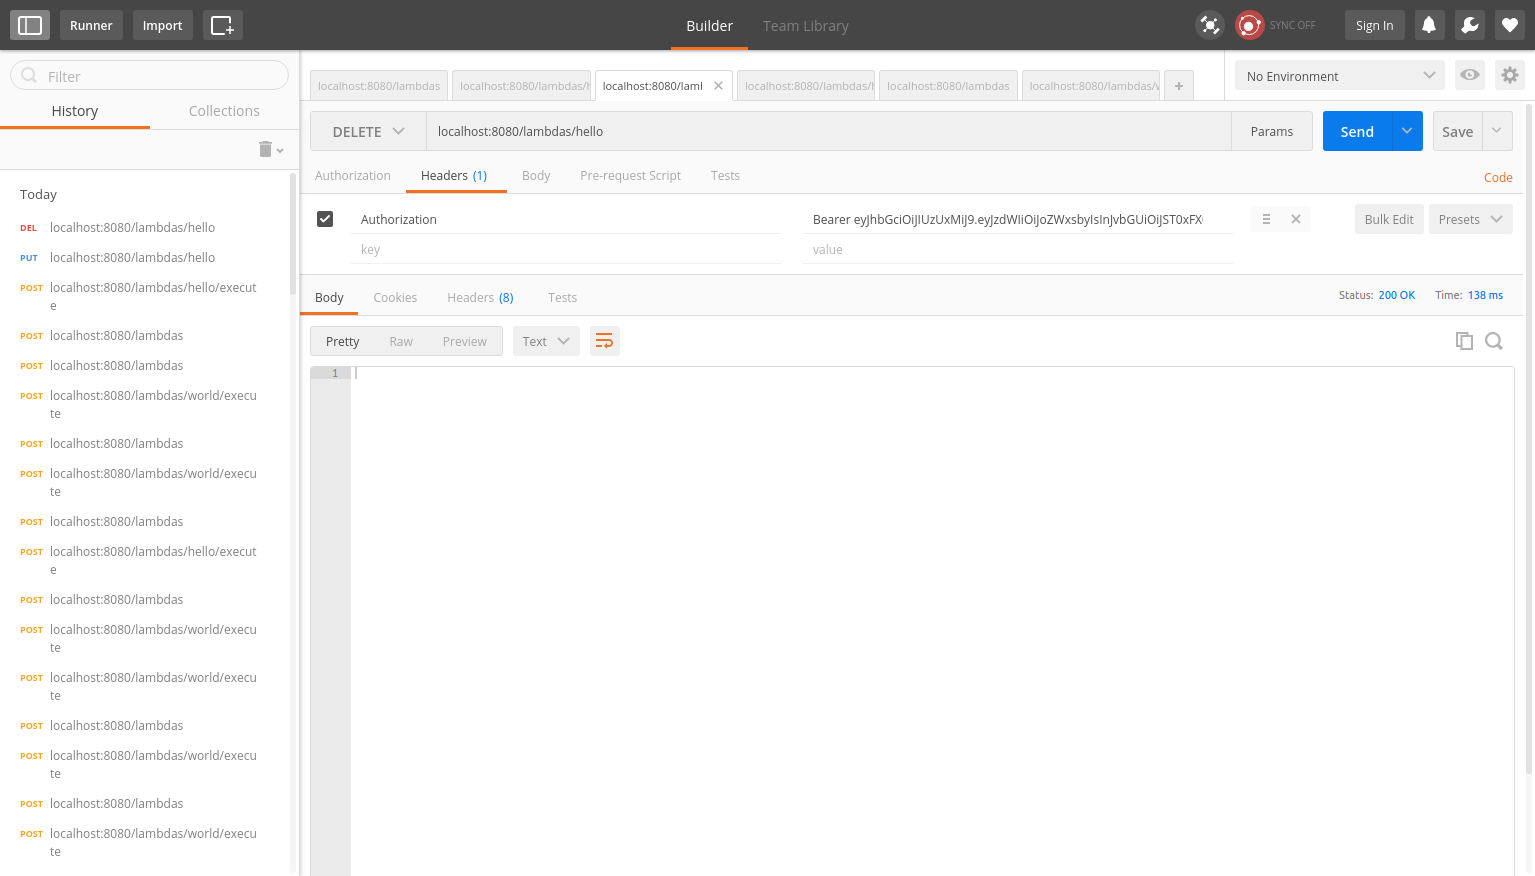
\includegraphics[width=\textwidth]{delete.png}
	\section{Lambda ausführen}
	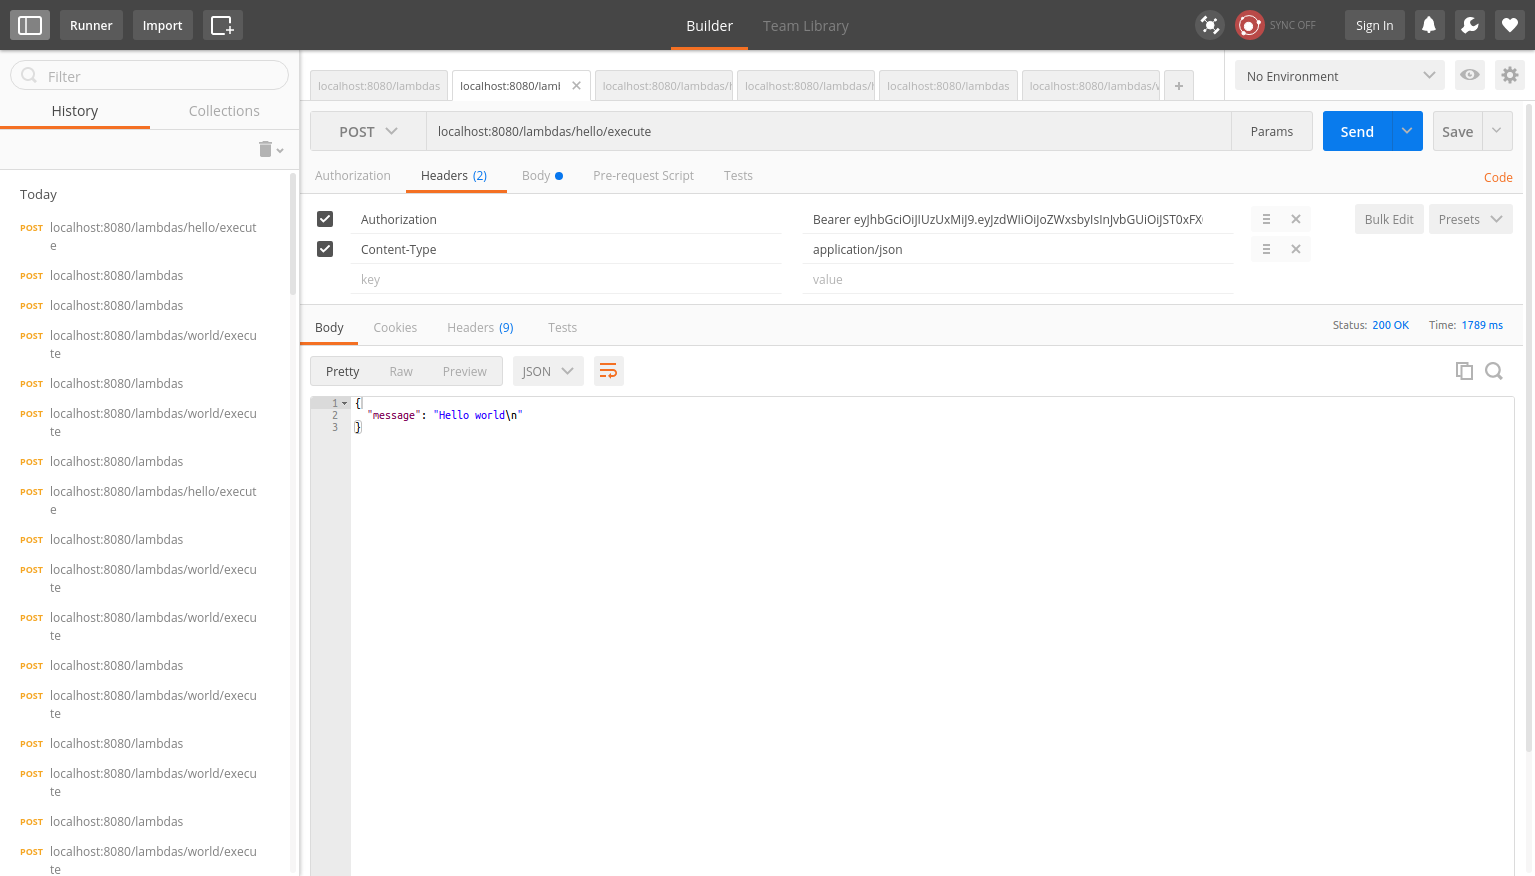
\includegraphics[width=\textwidth]{execute.png}
	\chapter{Vergleich der implementierten Funktionen mit der Definition aus dem Pflichtenheft}
	\section{Erfüllung der Musskriterien}
	\subparagraph{Musskriterien funktionaler Art}
	\begin{itemize}
		\item[$\surd$] Der Lambda-Entwickler soll die Lambda-Funktion mithilfe einer einfachen REST-API hochladen können.
		\item[$\surd$] Der Lambda-Entwickler soll die Lambda-Funktion mithilfe einer einfachen REST-API ausführen können.
		\item[$\surd$] Der Lambda-Entwickler soll die Lambda-Funktion mithilfe einer einfachen REST-API löschen können.
		\item[$\surd$] Der Lambda-Entwickler soll die Lambda-Funktion mithilfe einer einfachen REST-API ändern können.
		\item[$\surd$] Der Lambda-Entwickler soll die Lambda-Funktion mithilfe einer einfachen REST-API benennen können.
		\item[$\surd$] Die Konfigurationen (z.B. Signatur, Funktionsparameter, Ausführungsanzahl) der Lambda-Funktion sollen spezifiziert werden können.
		\item[$\surd$] Der Lambda-Entwickler sollen mithilfe eines Tokens authentifiziert werden können.
		\item[$\surd$] Lambda-Verwender sollen mithilfe eines Tokens, der vom Lambda-Entwickler ausgegeben wird authentifiziert werden können und mit diesem Token Lambda-Funktionen ausführen.
		\item[-] Laufende Instanzen gelöschter Lambda-Funktionen sollen gestoppt werden.
		\item[$\surd$] Lambda-Funktionen sollen zustandslos sein.
		\item[$\surd$] Lambda-Funktionen sollen gekapselt werden.
		\item[$\surd$] Lambda-Funktionen dürfen nur eine vom Server spezifizierte Zeit lang laufen.
	\end{itemize}
	\subparagraph{Musskriterien nichtfunktionaler Art}
	\begin{itemize}
		\item[$\surd$] Das System soll in Rechner- und Speicherressourcen skalierbar sein.
		\item[$\surd$] Das System soll um Sprachen für Lambda-Funktionen erweiterbar sein. //Dynamisches Laden von Sprachen wurde implementiert.
	\end{itemize}
	\section{Erfüllung der Wunschkriterien}
	\subparagraph{Wunschkriterien funktionaler Art + erweiterte Funktionen}
	\begin{itemize}
		\item[-] Lambda-Entwickler sollen eine Höchst-Laufzeit spezifizieren können, die nicht die maximale Laufzeit überschreitet.
		\item[-] Zu jedem Token wird ein Zähler erstellt, der für statistische Zwecke ausgelesen werden kann.
		\item[-] Der Lambda-Entwickler können ein Repository angeben und von dort die Lambda-Funktion auf den Server laden.
		\item[-] Versionsverwaltung für hochgeladene Lambda-Funktionen.
		\item[-] der Server kann Firewall-Einstellungen für Lambda-Funktionen definieren.
		\item[-] Der Lambda-Entwickler können Firewall-Einstellungen für Lambda-Funktionen definieren, sofern sie nicht den Server-Einstellungen widersprechen.
		\item[-] Sofern die Ausführungszeit einer die Lambda-Funktion ein Limit überschreitet, wird die HTTP-Verbindung abgebrochen und bei Beendigung der Lambda-Funktion wird das Ergebnis bereitgestellt.
		\item[?] Prepaid-Bezahlsystem für Tokens. //ein Bitcoin-System wird implementiert.
		\item[-] spätere Bereitstellung des Ergebnisses für Lambda-Funktion.
		\item[-] Der Serverbetreiber kann Statistiken einsehen.
	\end{itemize}
	
	\subparagraph{Wunschkriterien nichtfunktionaler Art}
	\begin{itemize}
		\item[$\surd$] Die Ausführung einer stark ressourcenaufwändigen die Lambda-Funktion beeinträchtigt nicht die Ausführung anderer Lambda-Funktionen auf dem Server.
	\end{itemize}
	
	\section{Erfüllung der Abgrenzungskriterien}
	\begin{itemize}
		\item[-] Entwicklung einer graphischen Nutzeroberfläche.
		\item[-] Entwicklung einer Nutzerverwaltung mit Datenbank. //nicht notwendig, da alle Nutzerinformationen in den Tokens gespeichert werden.
	\end{itemize}
	\printglossaries
\end{document}
